\documentclass[10pt,twocolumn,letterpaper]{article}

\usepackage{cvpr}
\usepackage{times}
\usepackage{epsfig}
\usepackage{graphicx}
\usepackage{amsmath}
\usepackage{amssymb}
\usepackage{float}
\restylefloat{table}

% Include other packages here, before hyperref.

% If you comment hyperref and then uncomment it, you should delete
% egpaper.aux before re-running latex.  (Or just hit 'q' on the first latex
% run, let it finish, and you should be clear).
\usepackage[breaklinks=true,bookmarks=false]{hyperref}

\cvprfinalcopy % *** Uncomment this line for the final submission

\def\cvprPaperID{****} % *** Enter the CVPR Paper ID here
\def\httilde{\mbox{\tt\raisebox{-.5ex}{\symbol{126}}}}

% Pages are numbered in submission mode, and unnumbered in camera-ready
%\ifcvprfinal\pagestyle{empty}\fi
\begin{document}

%%%%%%%%% TITLE
\title{Recognizing Multiple Classes Using One-vs-All Classification and Ensembles}

\author{Thomas Aurigemma\\
University of Massachusetts, Amherst\\
Amherst, MA 01003\\
{\tt\small taurigemma@umass.edu}
% For a paper whose authors are all at the same institution,
% omit the following lines up until the closing ``}''.
% Additional authors and addresses can be added with ``\and'',
% just like the second author.
% To save space, use either the email address or home page, not both
\and
Liam Rothschild-Shea\\
{\tt\small lrothschilds@umass.edu}
}

\maketitle
%\thispagestyle{empty}

%%%%%%%%% ABSTRACT
\begin{abstract}
   This project was conducted to observe the performance of a set of one-vs-all classifiers working together as an ensemble to classify images. The minimum number of classes required in an image classification problem is two. The more classes introduced makes achieving high accuracies more difficult, therefore the easiest image classification problems are ones only consisting of two classes. Any image classification problem can be broken down into a set of classification problems, classifying whether an image is or is not a member of a specific class. The proposed structure aims to convert any image classification problem into the suggested set to utilize the simplicity of a two-class image classification problem on a dataset with more than two classes. The model sends the data to several different convolutional neural networks (CNN), each uniquely designed to act as a one-vs-all classifier for a specific class. The results of each of the one-vs-all classifiers are combined where an image can fall under one of two cases. If one or more of the one-vs-all classifiers recognizes the image as a member of that class, the image is given the label corresponding to the class that is most sure of that membership. If an image is not recognized by any of the one-vs-all classifiers the image remains unlabeled and is considered an incorrect prediction. The prediction is then compared against the image’s true class. This structure theoretically can perform at least as well as a standard CNN can as an  image classifier, however, due to the significantly higher development and runtime requirements this is not a better option than a traditional approach to image classification.
\end{abstract}

%%%%%%%%% BODY TEXT
\section{Introduction}
Image classification is a task that convolutional neural networks are well suited to complete. A CNN has the ability to learn both high- and low-level features of a set of images and use those features to classify images it has never seen before. Neural networks that are tasked with recognizing many different classes often have much more complex architectures to enable them to recognize all classes with high accuracy. The neural network needs to be able to learn many different features from all the separate classes, requiring the network to have an overall higher capacity to learn. For this project, we attempted to create a new framework to improve upon normal image classification.

When using an ensemble of neural networks, a set of neural networks are trained to classify images of various classes and when an image is input into the ensemble to be classified, each neural network produces a potential label for the image. One label is selected from the multiple outputs and is used as the final label for the image. Our framework proposes an overall similar structure, but instead of every network being trained to recognize all classes, each network is trained as a one-vs-all network that can recognize only a single class. The results of each network are then combined to produce a final label for each input image. This structure of neural networks was proposed due to many potential benefits over a standard neural network or ensemble, such as allowing for performance for a single class to be easily fine tuned without affecting the performance of other classes and the ability for one-vs-all classifiers to recognize each class with high accuracy while having relatively simple architectures. Throughout this paper we will discuss our implementation of this structure, the performance results we achieved, and analyze the merit of this concept and whether or not further investigation and research should be completed.

\begin{figure*}
	\begin{center}
	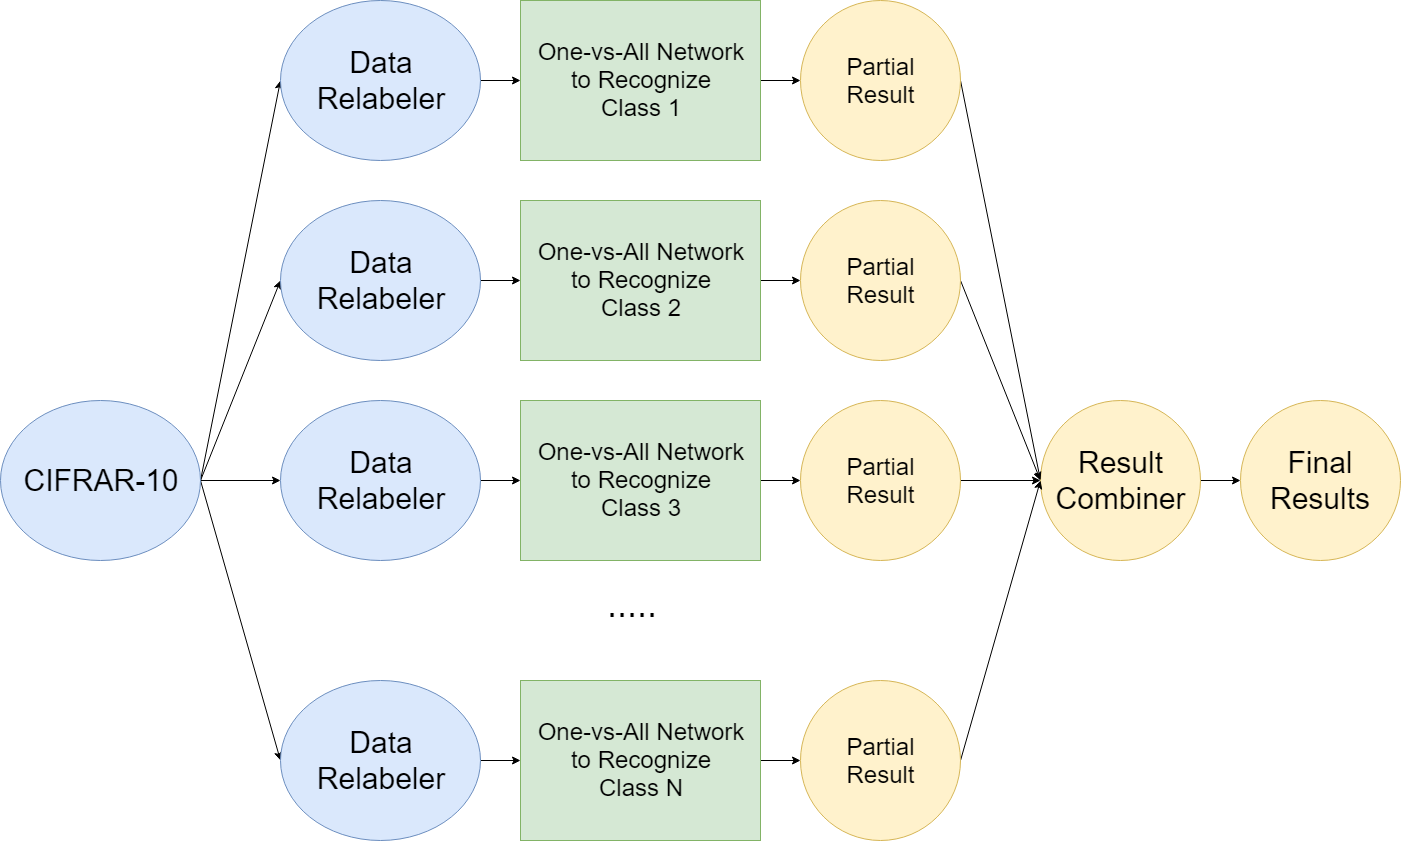
\includegraphics[width=12cm,height=6cm]{architecture_revised.png}
	\end{center}
	\caption{Simplified Model Visualization}
\end{figure*}

\section{Background/Related Work}
Standard ensembles of neural networks are well known to increase overall performance. In \textit{The Relative Performance of Ensemble Methods with Deep Convolutional Neural Networks for Image Classification} [1] the authors Ju, Bibaut, and van der Laan discuss the benefits of using multiple neural networks to solve a single classification problem and different ways to analyze the results of a set of neural networks. This information is relevant to this project because at test time the proposed structure will produce one set of results per class, similar to how an ensemble will produce one set of results per network. Two of the techniques the authors discuss to combine the different outputs include using an unweighted average of the sets of results as the final results and using a voting system to produce a set of results based on the most common output labels. While neither of these approaches can be directly applied to the set of one-vs-all classifiers, they give useful insight into how to combine multiple sets of results in a mathematical manner.

In \textit{In Defense of One-Vs-All Classification} [2] the authors Rifkin and Klautau argue that using a set of one-vs-all classifiers to classify an entire dataset will achieve performance at least as good as that of other types of classifiers and is therefore useful due to its computational and conceptual simplicity. Rifkin’s and Klautau’s work is relevant to this project because they created a similar one-vs-all classification structure to solve a classification problem and they reported relative success in their investigation. The authors comment on results of previous experiments, stating that the one-vs-all classifiers that were used were not accurate enough and if “a reasonable effort was made to find correct settings for the hyperparameters of the algorithm … and that the best available binary classifiers are used” then a set of binary classifiers should perform at least as well, if not better than other approaches to the same problem. The authors demonstrate their argument by solving the same classification problem using both one-vs-all classification and all-vs-all classification and were successful in achieving similar results with both approaches to the problem.

There are many commonly used datasets to test image classification. High levels of performance have been achieved by various different neural networks for most commonly used datasets. In \textit{Generalizing Pooling Functions in Convolutional Neural Networks: Mixed, Gated, and Tree} [3] the authors Lee, Gallagher, and Tu report that they were able to achieve 92.38\% accuray on the Cifar-10 dataset. They were able to improve their accuracy even further to 93.95\% by augmenting the data to increase the size of the dataset. In \textit{Fractional Max-Pooling} [4], author Benjamin Graham is able to achieve 96.53\% accuracy on the Cifar-10 dataset using a convolutional neural network and a modified pooling layer. These results are important to note because they provide a point of reference to compare the performance of the ensemble of one-vs-all classifiers against. For the results of this project to be considered successful, the performance of the networks must not only be high, but it must be at least similar to that of other validated methods.

\section{Approach}
Our project requires several one-vs-all classifiers to learn to recognize a single class, so the dataset must first be modified to be able to be input into each network. First, the dataset is read in and a copy is made for each class in the dataset. The copies of the training, validation, and testing labels for each dataset are then rewritten such that every image of the corresponding class is assigned a label of one and every other image is given a label of a zero. Each copy of this dataset is then input into its corresponding one-vs-all convolutional neural network and each network is trained until performance has converged. The architecture, layers, weight initialization, and optimizers for each one-vs-all network vary, but all architectures contain multiple convolutional layers and all networks use the cross-entropy loss function. Once training has finished, the test images are input into each network and a set of labels is output for each network. Since each network is capable of only recognizing a single class, the results from all the neural networks must be combined to create a complete set of labels that can be used to assess overall performance of the set of classifiers.

There are many ways to combine the sets of results but the one that was selected for this project works as follows. If only a single one-vs-all classifier recognizes an image, then it is used as the final label for the image. If multiple one-vs-all classifiers recognize the same image, then the scores from each potential labeling are analyzed to give the best possible guess for the final label. The scores of an image are converted into normalized probabilities for each potential class. By calculating the normalized probabilities for each class, the proposed label with the highest probability can be selected. In short, the network that assigns the highest confidence to its labeling is chosen to provide the final label. If an image is not recognized by any of the one-vs-all classifiers, then there are no proposed labelings so the image cannot be given a label. The image is instead given a “garbage” label, which is simply a label associated with no class in the dataset. This means the image will be marked as incorrect when assessing the performance of the ensemble.

Figure 1 provides a simplified visualization of the ensemble of one-vs-all classifiers.. The data is relabeled and input into each network so that they can learn a specific class independently of every other network. Each network outputs its own set of results which are then combined into one final set of results that are used to assess performance.

\section{Experiment}
The dataset used to realize this approach was the Cifar-10 dataset [5]. The Cifar-10 dataset is composed of 60,000 (50,000 training and 10,000 testing) 32x32x3 real images, each belonging to one of ten classes: airplane, automobile, bird, cat, deer, dog, frog, horse, ship, and truck. Each image is paired with a label which is equivalent to the images corresponding class. The proposed approach is not conceptually bound to any image dataset as it aims to address image classification and since the run time directly impacts how long it takes to process and handle an image, a dataset composed of small color images would function well as a test case. This dataset is also freely available online, ensuring  the validity of the data itself as it is a widely renowned and used dataset for testing methods of image classification.

The ensemble began as multiple instances of a single CNN, each trained to act as a one-vs-all classifier for each of the ten possible classes an image could belong to. Once every network had been trained and tested, the predictions from each of the one-vs-all classifier test runs were combined. The ensemble would then label the image with the class corresponding to a random one-vs-all classifier that recognized the image. If the image was not recognized by all the one-vs-all classifiers then the ensemble would assign the image with the “garbage” label, essentially leaving the image as “unlabeled”. Any unlabeled image was valued as an incorrect labeling, and these combined predictions were considered the results of the ensemble.

The architecture of the set of classifiers was trivial and the method of selecting a final prediction was arbitrary so the initial results functioned as a baseline and the overall structure of the ensemble became a starting point. Randomly selecting the label for an image from the set of classifiers that recognized it has little mathematical benefits over a more robust system. Each one-vs-all classifier returned a set of scores for every image that can be converted to probabilities for each class. This fact led the decision process to be changed to the following; the results of all ten one-vs-all classifiers are combined and if none of the classifiers labeled a specific image as true, that image is labeled "unlabeled". If one of the classifiers labeled a certain image as true and the rest of the classifiers labeled it as false, the image is predicted to be the class corresponding to the one-vs-all classifier that labeled it as true. Otherwise, more than one of the classifiers labeled a specific image as true. The image is predicted to be the class corresponding to the one-vs-all classifier that had the  greatest probability of the image being a member of that class. This update in the prediction method was observed to improve overall performance by 1.79\%.

With the prediction method update completed, the next step was to modify the architecture of the one-vs-all classifier. The network was originally composed of a two-dimensional convolution followed by a rectified linear unit (ReLU) activation and a single affine layer. The network did not use any form of weight initialization and had stochastic gradient descent (SGD) as an optimizer. Instead of modifying and then training this model for all classes, it was decided to first modify it to perform well for one class and then determine how well that model functions for each class. The original architecture performed best when classifying automobiles, so its was modified to perform as well as possible for recognizing automobiles. The automobile architecture became a nine-layer neural network consisting of eight two dimensional convolutions, eight ReLU activations, four two-dimensional max pool layers, and four dropout layers. The more complex architecture greatly improved performance, however the network was held back by the loss function not going down quickly enough. To fix this, the optimizer of the network was changed from SGD to RMSprop with a learning rate of 0.0005, which decreased the loss value and resulted in a higher accuracy. An initialization method was implemented  as the results showed to be inconsistent across multiple tests and the training process would rarely crash due to an exploding loss function. Xavier normalization was chosen as the initializer for the automobile network, and the results were immediately more consistent and there were no longer issues with an exploding or disappearing loss function.

The automobile network was able to consistently achieve an accuracy of above 97\% when acting as a binary classifier on the test set. This was not the case, however, when analyzing the performance of the automobile network as a binary classifier for each class. None of the other classes were able to achieve an accuracy over 97\%, even with tweaking all the different parameters of the network. This led to the creation of a second one-vs-all classifier, but since the classifier recognized ships with the highest accuracy out of the remaining nine one-vs-all classifier for ships. The initialization method and optimizer were kept the same, but by removing all the dropout calls and keeping the rest of the architecture (down to the parameters) the same as the automobile network, the network achieved an accuracy of 96\% when acting as a binary classifier on the test data. Testing the new ship network on the remaining eight classes produced results similar to that of the automobile network as it was not able to achieve an accuracy over 95\% when acting as binary classifier for any of the other classes. This evident pattern confirmed the notion that to achieve the best combined results possible, each one-vs-all classifier would have to be developed and fine tuned individually. Given an already established model performed well on a new class, it acted as a foundation to be modified to attain better results for that class, but if the model did not perform well on a class, a completely new and independent architecture was created.

\begin{figure}[H]
	\begin{table}[H]
	\centering
		\begin{tabular}{llll}
			\textbf{Class} & \textbf{Accuracy (\%)} & \textbf{} & \textbf{} \\
			Airplane       & 95.36                  &           &           \\
			Automobile     & 97.74                  &           &           \\
			Bird           & 93.01                  &           &           \\
			Cat            & 91.45                  &           &           \\
			Deer           & 93.98                  &           &           \\
			Dog            & 94.14                  &           &           \\
			Frog           & 94.47                  &           &           \\
			Horse          & 95.38                  &           &           \\
			Ship           & 96.71                  &           &           \\
			Truck          & 95.83                  &           &           \\
			Combined       & 68.04                  &           &          
		\end{tabular}
	\end{table}
	\caption{Results of Automobile Classifier Trained For All Classes}
\end{figure}

This realization led to the creation of the following process. The first step was to test all existing networks on a class that does not have an already existing classifier. If at least one of the networks produced a high accuracy (generally above 92\%) on the test data, whichever network that produced the highest accuracy was used as the foundation for that classifier. Once the foundation had been chosen, modifications to the parameters and overall architecture were be made. If none of the existing networks performed admirably as a one-vs-all classifier on the test data for this class, then the classifier was built from scratch. In both cases, the goal was to push the accuracy of the networks to 95\% on the test set. One of two initialization methods, Xavier and Kaiming, and one of two optimizers, Adam and RMSprop, were used for each of the networks, however, the learning rate of the optimizers differed from network to network. The distinct layers used over all the networks were two-dimensional convolutional and two-dimensional convolutional transpose layers, two-dimensional max pool layers, dropout layers, two-dimensional and one-dimensional batch normalization layers, and a combination of ReLU, Leaky ReLU, and ELU activation functions.

As mentioned above, once the automobile network was established, its architecture was used as the base for the ship network. Once the ship network was improved to produce over 95\% accuracy on the test data, work began on the truck network starting from scratch since neither the automobile nor ship network had an accuracy over 92\% when used as a binary classifier for trucks. The airplane network followed suit, as once the truck network was complete, none of the three existing networks functioned well as a one-vs-all classifier for airplanes. The horse network was also built from scratch, however that network was able to achieve an accuracy over 95\% for the frog class without any modifications so it was used as the classifier for frogs as well. The bird network had to be built from scratch as well, but it performed well enough as a classifier for dogs and deer, so it also functioned as a template for those respective classes. Modifications were made to the dog network by changing out all ReLU activations with Leaky ReLU activations and by adding an additional one-dimensional batch normalization layer. These alterations produced an accuracy over 95\% when classifying images of dogs, and when the same changes were applied to the deer network the same increase in accuracy was observed. The cat network was the last network to be finalized, as it proved to be the most difficult to obtain high accuracy on. When a network’s structure was used as the base for another classifier, the initialization method and optimizer were carried over as well. The original initializer and optimizer (including learning rate) remained the best option for classifiers when using another network as a base. This process produced the best performance for all the classifiers.

To effectively evaluate the final test results, the accuracies of each of the one-vs-all classifiers were tracked along with the overall accuracy of the ensemble on the test data. To test the validity of this structure against a standard approach to image classification, we designed a standard CNN to compare the test accuracy against. The CNN is thirteen layers deep and recognizes images from all ten classes at once. This network utilized the ReLU activation function between every layer and dropout and batch normalization were alternatingly used in between each layer. A max pooling layer was used after every fourth convolution.

The total number of unlabeled images produced by the ensemble was collected to assess how unlabeled images affect the results, as well as the number of unlabeled images produced per class to see how the individual accuracies of each network affected the number of unlabeled images for that class. An image that not recognized by the classifier corresponding to the true class of the image is considered a false negative prediction by the ensemble. The only way an image can go unlabeled is if it is predicted as a false negative by its respective classifier and every other classifier does not recognize it. Analysis of which images are frequently considered false negatives by their respective class can provide insight into which images are consistently going unlabeled by the ensemble, so a set of false negative images was produced to give a window into the issues caused by unlabeled images. A false positive prediction occurs when an image is recognized by a classifier not matching the class of the image. During the process of combining the results, images that were recognized by multiple classifiers are said to have a collision.  Collisions can only occur if the image is recognized by the classifier matching the class of the image and at least one other classifier predicted that image as a false positive, or the image is classified as a false negative by its respective classifier and at least two other classifiers predicted that image as a false positive. Due to false negatives relationship to collisions an image set was created to show examples of false negatives produced by the ensemble for each class.

\begin{figure}[H]
	\begin{table}[H]
		\begin{tabular}{llll}
			\textbf{Class} & \textbf{\begin{tabular}[c]{@{}l@{}}Test\\ Accuracy\end{tabular}} & \textbf{\begin{tabular}[c]{@{}l@{}}No.\\ Unlabeled\end{tabular}} & \textbf{\begin{tabular}[c]{@{}l@{}}\% of Total\\ Unlabeled\end{tabular}} \\
			Airplane       & 95.73                                                            & 270                                                              & 13.20                                                                    \\
			Automobile     & 97.62                                                            & 117                                                              & 5.72                                                                     \\
			Bird           & 95.08                                                            & 160                                                              & 7.82                                                                     \\
			Cat            & 93.09                                                            & 327                                                              & 15.99                                                                    \\
			Deer           & 96.33                                                            & 157                                                              & 7.68                                                                     \\
			Dog            & 95.54                                                            & 180                                                              & 8.80                                                                     \\
			Frog           & 96.29                                                            & 184                                                              & 9.00                                                                     \\
			Horse          & 96.29                                                            & 285                                                              & 13.94                                                                    \\
			Ship           & 96.76                                                            & 185                                                              & 9.05                                                                     \\
			Truck          & 96.88                                                            & 180                                                              & 8.80                                                                    
		\end{tabular}
	\end{table}
	\caption{One-vs-All Classifier Results}
\end{figure}

The final ensemble achieved an accuracy of 71.01\% on the 10,000 test images.  Each of the one-vs-all classifiers was able to achieve an accuracy over 95\%, except for the classifier designed to recognize cats which achieved an accuracy of 93.09\%. A lot of time was spent pushing this classifier to achieve an accuracy above 93\%. As mentioned, the goal was to have each individual classifier attain an accuracy over 95\%. Some networks were faster to build as their they reached accuracies above 95\% with ease, while others took significant amounts of time to develop and finetune, but they still were able to get accuracies above 95\%. Once the other nine networks passed the threshold of 95\% accuracy and a significant amount of time was spent increasing the performance of the cat classifier from 91\% to 93\%, we decided that the classifiers were accurate enough to collect results and draw conclusions from. Treating this network as an outlier, the average performance of the five remaining networks was 96.28\% with accuracy ranging from 95.08\% (bird classifier) to 97.62\%(automobile classifier). The standard CNN that was constructed was able to achieve an accuracy 81.03\% on the test data.

When passed through the ensemble, 2,045 of the 10,000 test images went unlabeled. Since these cases are treated as an incorrect prediction, this reduced the overall accuracy of the ensemble by 20.45\%.  This means that excluding unlabeled images, the ensemble correctly label an image with an accuracy of 89.26\%. This signifies unlabeled images as the main cause for significantly lower overall accuracy. Of the 2045 unlabeled images, 327(15.99\%) of them were images of cats. The average number of unlabeled images of the other nine classes is 191(9.34\%), rounding up to the next integer. This shows that not being able to push the cat classifier as far as the other classifiers significantly reduced overall accuracy.

\begin{figure}[H]
	\begin{center}
		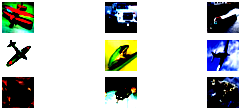
\includegraphics[width=6cm,height=4cm]{SomeFalsePositives.png}
	\end{center}
	\caption{Subset of False Positive Images}
\end{figure}

The false positive image set shows images of birds frequently being mislabeled as airplanes and vice versa. This relationship between two classes can also be seen between automobiles and trucks. It makes logical sense for birds and airplanes to be confused for one another, and automobiles and trucks to be confused, due to the pairs sharing similar colors, shapes, backgrounds, and many more features. The green and yellow image of a frog in Figure  4 was incorrectly labeled a bird when looking at the false positive set. This frog has a similar position and background to many images of birds. This is also true for the image of a horse in the center of Figure 5 that was considered a false positive by the classifier for the truck class. Both these images, while they did not go unlabeled, still contributed to a loss in accuracy as they were considered both false negatives by their own classifier and false positives by another.

\begin{figure}[H]
	\begin{center}
		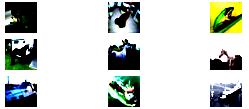
\includegraphics[width=6cm,height=4cm]{SomeFalseNegatives.png}
	\end{center}
	\caption{Subset of False Negative Images}
\end{figure}

\section{Conclusion}
We were able to successfully produce an ensemble of ten (one per class) one-vs-all classifiers, each with over 95\% accuracy on the test data, except for one that achieved about 93\%. However, when the results are combined to act as a standard classifier the accuracy drops to approximately 71\% due in large part to 20\% of the images receiving no label. When compared to pre-existing models that have been applied to the Cifar-10 dataset such as the model created by Lee, Gallagher, and Tu that achieved an accuracy of 92.83\% and the model created by Benjamin Graham which achieved 96.53\%, our results are significantly worse.  When compared to the standard CNN that we built, which was able to achieve an accuracy of 81\% on the Cifar-10 dataset, our results look even less promising. The standard CNN was developed faster than each one-vs-all classifier, making the ensemble appear to be an inferior option in comparison. The image sets are useful sanity checks, as they show that images are only being misclassified in cases where it makes visual sense for the images to be mixed up. The high number of false negatives is the cause behind the large number of unlabeled images which in turn is the cause of the much lower accuracy of the ensemble. Every percent gained by pushing the accuracies of the individual one-vs-all classifiers closer to 100\% decreases the number of unlabeled images by a notable amount, which in turn increases the accuracy of the network by a large margin. The set of classifiers performs well (89\%) at labeling an image, given that the image is recognized by any of the classifiers. However, as we experienced, it is inefficient to spend an inordinate amount of time and effort pushing one classifier in the entire ensemble to achieve 1\% better performance while a fraction of that time and effort can be spent achieving 10\% higher accuracy on the test data by using a standard classifier.

The simplest improvement that can be made is further fine tuning of the individual one-vs-all classifiers. Given enough tweaking and fine tuning, this structure should be able to attain better results, eventually approaching the performance achieved by other models. Performance increases specifically to the cat network should significantly increase overall performance. Replacing our own one-vs-all classifiers with fine tuned, pretrained image classifiers may lead to an increase in performance for some classes. There are many available pre-trained models that perform well as image classifiers, and a pre-trained image classifier has the potential to have high accuracy when functioning as a one-vs-all classifier on the same data.

An alternative to allowing an image to go unlabeled is to input all unlabeled images into a standard image classifier, so that all images will receive a label. This would immediately produce a large increase in accuracy assuming the standard classifier had a high accuracy. The caveat to this is that if the network that is being used to rectify unlabeled images performs significantly better than the ensemble, then the argument can be made that a similar or higher accuracy could be achieved if the standard network alone was used to classify all the images. Also, while this modification would increase the performance of the structure on the test data, it introduces yet another network to the model, further increasing complexity, training time, and testing time.

Replacing each one-vs-all classifier with a traditional ensemble of one-vs-all classifiers may also help improve performance. Multiple one-vs-all classifiers could be created and trained to recognize each class and the results for each class could be combined into a single set of intermediary results using either the unweighted averaging system or the voting systems previously discussed. The intermediary results for all classes could then be input into one of the combining systems used by the normal one-vs-all structure discussed previously. Replacing each network with an ensemble should increase per-class accuracy and therefore increase overall accuracy. However, this potential increase in accuracy does have a cost. Using an ensemble in place of each one-vs-all classifier would increase the amount of networks to be designed, tuned, and trained significantly and testing runtime would be increased even further.

In the work done by Lee, Gallagher, and Tu,  they were able to increase the accuracy of their classifier on the Cifar-10 dataset by implementing data augmentation [3]. This method could be used to increase the size of the input dataset, which in turn may help each classifier to learn to recognize its designated class with higher accuracy. The set of one-vs-all classifiers could also be trained to recognize another dataset with a different set of classes, which could allow for a more thorough analysis of the effectiveness of this structure.

We tested many different architectures, optimizers, and initializations when designing the classifiers, but a significant amount of improvement must be done before overall performance surpasses that of other established image classification methods. Fortunately, there are many different obvious improvements that can be made that should significantly increase performance, meaning continued work has high potential to improve on this model. Despite this potential, we must conclude that this modified ensemble of one-vs-all classifiers is not currently as effective as many other approaches to image classification.


{\small
\begin{thebibliography}{9}
\bibitem{1}
C. Ju, A. Bibaut, and M. J. van der Laan, “The Relative Performance of Ensemble Methods with Deep Convolutional Neural Networks for Image Classification”, ArXiv e-prints, Apr. 2017.

\bibitem{2}
R. Rifkin and A. Klautau, “In Defense of One–Vs-All
Classification”, Journal of Machine Learning Research 5
(2004) 101-141.

\bibitem{3}
Lee, C.Y., Gallagher, P.W. and Tu, Z., "Generalizing Pooling Functions in Convolutional Neural Networks: Mixed, Gated, and Tree", arXiv preprint arXiv:1509.08985 (2015) 

\bibitem{4}
Graham, Benjamin, "Fractional Max-pooling", In arxiv:cs/arXiv:1412.6071, 2015.

\bibitem{5}
Krizhevsky, A., “Learning Multiple Layers of Features from Tiny Images”, Master’s thesis, Department of Computer Science, University of Toronto, 2009.

\end{thebibliography}
}

\end{document}
